\mySection{6.2 The Decision Rule}
%-------------- start slide -------------------------------%{{{ 1
\begin{frame}[fragile]
 \begin{center}
 \begin{minipage}{0.6\textwidth}
 \begin{center}
Go over the example first....
\end{center}
 \end{minipage}
\end{center}
\end{frame}
%-------------- end slide -------------------------------%}}}
%-------------- start slide -------------------------------%{{{ 1
\begin{frame}[fragile]
 \begin{center}
 \begin{minipage}{0.6\textwidth}
 \begin{center}
    Suppose our friend Jory claims that he has some magic power to predict the side of a randomly tossed fair-coin.
    \bigskip

    Jory claims that he could do more than\\ $\textcolor{magenta}{1/2}$ \\ of the time on average.
    \bigskip

    Let's test Jory to see if we believe his claim.
\end{center}
 \end{minipage}
\end{center}
\end{frame}
%-------------- end slide -------------------------------%}}}
%-------------- start slide -------------------------------%{{{ 1
\begin{frame}[fragile]
 \begin{center}
 \begin{minipage}{0.6\textwidth}
 \begin{center}
    We made Jory guess a repeatedly tossed coin for 100 times.
    \bigskip

    He guesses correctly 54 times.
    \bigskip
    \bigskip

    {\bf  Question: }\\

    Does this provide strong evidence that Jory has the proclaimed magic power?
\end{center}
 \end{minipage}
\end{center}
\end{frame}
%-------------- end slide -------------------------------%}}}
%-------------- start slide -------------------------------%{{{ 1
\begin{frame}[fragile]
 \begin{center}
 If Jory is guessing randomly,  the number of correct guesses would follow a binomial distribution
 with parameters $n=100$ and $p=1/2$.
 \bigskip
 \bigskip

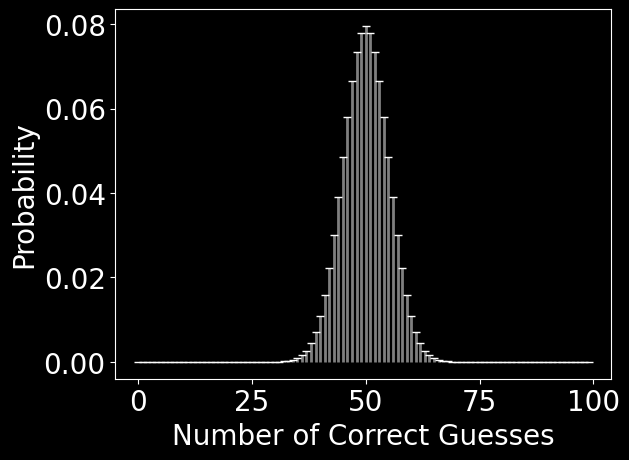
\includegraphics[scale=0.4]{Codes/Binomial_Jory.png}

\end{center}

\end{frame}
%-------------- end slide -------------------------------%}}}
%-------------- start slide -------------------------------%{{{ Guess 54
\begin{frame}[fragile]
\def\guess{54}
\def\ans{0.2421}
  \begin{center}
    What is probability that Jory gets \textcolor{red}{\guess\: or more} correct when guessing randomly?
 \bigskip
  \pause

 \includegraphics[scale=0.4]{Binomial_Jory_\guess.png}
  \end{center}
\bigskip
\begin{align*}
  \bbP\left(X\ge \guess\right) = \sum_{n=\guess}^{100} \binom{100}{n} \left(\frac{1}{2}\right)^n \left(\frac{1}{2}\right)^{100-n} = \textcolor{red}{\ans}.
\end{align*}
 \end{frame}
%-------------- end slide -------------------------------%}}}
%-------------- start slide -------------------------------%{{{ 54: Conclusion
\begin{frame}[fragile]
 \begin{center}
 \begin{minipage}{0.6\textwidth}
 \begin{center}
  It is not unlikely to get this many correct guesses due to chance.

  \bigskip
  \bigskip

  {\bf Conclusion:}\\
  \bigskip

  There is No strong evidence that Jory has better than a $1/2$ chance of correctly guessing the coin.

\end{center}
 \end{minipage}
\end{center}
\end{frame}
%-------------- end slide -------------------------------%}}}
%-------------- start slide -------------------------------%{{{ Guess 60
\begin{frame}[fragile]
\def\guess{60}
\def\ans{0.0284}
  \begin{center}
    What is probability that Jory gets \textcolor{red}{\guess\: or more} correct when guessing randomly?
 \bigskip
  \pause

 \includegraphics[scale=0.4]{Binomial_Jory_\guess.png}
  \end{center}
\bigskip
\begin{align*}
  \bbP\left(X\ge \guess\right) = \sum_{n=\guess}^{100} \binom{100}{n} \left(\frac{1}{2}\right)^n \left(\frac{1}{2}\right)^{100-n} = \textcolor{red}{\ans}.
\end{align*}
 \end{frame}
%-------------- end slide -------------------------------%}}}
%-------------- start slide -------------------------------%{{{ 60: Conclusion
\begin{frame}[fragile]
 \begin{center}
 \begin{minipage}{0.6\textwidth}
 \begin{center}
 Either
 \bigskip

\textcolor{red}{Jory is purely guessing with probability of success of $\frac{1}{2}$, and we witnessed a very unusual event due to chance.}

  \bigskip \pause
  Or
  \bigskip

  \textcolor{green}{ Jory is truly having the magic power to guess the coin.}
  \bigskip \pause

\mySeparateLine

{\bf Conclusion:}\\[1em]

We have strong evidence against \\
\textcolor{red}{Red Hypothesis} \\[1em]

Or the test is in favor of \\
\textcolor{green}{Green Hypothesis}


% that Jory does have the magic power to do better than a $1/2$ chance of correctly guessing the coin.

\end{center}
 \end{minipage}
\end{center}
\end{frame}
%-------------- end slide -------------------------------%}}}
%-------------- start slide -------------------------------%{{{ 1
\begin{frame}[fragile]
 \begin{center}
 \begin{minipage}{0.6\textwidth}
 \begin{center}
  Before testing Jory, could you set up a threshold above which we will believe Jory's super power?
  \bigskip
  \pause

  Find smallest $\textcolor{red}{m}$ such that

\begin{align*}
  \bbP\left(X\ge \textcolor{red}{m}\right) = \sum_{n=\textcolor{red}{m}}^{100} \binom{100}{n} \left(\frac{1}{2}\right)^n \left(\frac{1}{2}\right)^{100-n} \le \textcolor{red}{0.05}
\end{align*}
\pause
\[\Downarrow\]
\begin{align*}
\boxed{m = 59}
\end{align*}
\small
b.c. $\bbP\left(X\ge 58\right)=0.067$ \& $\bbP\left(X\ge 59\right)=0.044$
  \end{center}
 \end{minipage}
\end{center}
\end{frame}
%-------------- end slide -------------------------------%}}}
%-------------- start slide -------------------------------%{{{ 1
\begin{frame}[fragile]
 \begin{center}
 \begin{minipage}{0.6\textwidth}
 \begin{center}
 We have just informally conducted a hypothesis test with the\\
 \textcolor{red}{null hypothesis}
 \begin{align*}
   \textcolor{red}{H_0: p=\frac{1}{2}}
 \end{align*}
 against the \\
 \textcolor{green}{alternative hypothesis}
 \begin{align*}
   \textcolor{green}{H_1: p>\frac{1}{2}}
 \end{align*}
 under the\\
 \textcolor{yellow}{significance level $\alpha=0.05$}\\[0.5em]
 which is equivalent to either \\[1em]
 \begin{minipage}{0.45\textwidth}
 \begin{center}
 producing the \\
 \textcolor{yellow}{critical region\\
 $m\ge 59$}
 \end{center}
 \end{minipage}
 \hfill or \hfill
 \begin{minipage}{0.45\textwidth}
 \begin{center}
 comparing with \\
 the \textcolor{yellow}{p-value.}
 \end{center}
 \end{minipage}
 \end{center}
 \end{minipage}
\end{center}
\end{frame}
%-------------- end slide -------------------------------%}}}
%-------------- start slide -------------------------------%{{{ 6.8
\begin{frame}
\begin{itemize}
  \item  \textcolor{magenta}{Test statistic:}
		Any function of the observed data whose numerical value
		dictates whether $H_0$ is accepted or rejected.
	\vfill
  \item  \textcolor{magenta}{Critical region} $C$:
		The set of values for the test statistic that result in
		the null hypothesis being rejected.\\[1em]
  \item[] \textcolor{magenta}{Critical value}:
		The particular point in $C$ that separates the rejection region from the acceptance region.
	\vfill
   \item \textcolor{magenta}{Level of significance} $\alpha$:
		The probability that the test statistic lies in the critical region $C$ under $H_0$.
\end{itemize}
\end{frame}
%-------------- end slide -------------------------------%}}}
%-------------- start slide -------------------------------%{{{ 6.9
\begin{frame}{Test Normal mean $H_0: \mu=\mu_0$ ($\sigma$ known)}

{\bf Setup:~}
\begin{enumerate}
 \item Let $Y_1=y_1,\cdots,Y_n=y_n$ be a random sample of size $n$ from $N(\mu,\sigma^2)$ with $\sigma$ known.
  \item Set $\bar{y}=\frac{1}{n}(y_1+\cdots+y_n)$ and $z=\frac{\bar{y}-\mu_0}{\sigma/\sqrt{n}}$.
 \item The level of significance is $\alpha$.
\end{enumerate}

\vfill\pause
{\bf Test:}\\
\begin{minipage}{0.3\textwidth}
 \[
 \begin{cases}
     H_0: \mu= \mu_0 \\
     H_1: \mu> \mu_0 \\
 \end{cases}
 \]
 reject $H_0$ if $z\ge z_\alpha$.
\end{minipage}
\hfill
\begin{minipage}{0.3\textwidth}
 \[
 \begin{cases}
     H_0: \mu= \mu_0 \\
     H_1: \mu< \mu_0 \\
 \end{cases}
 \]
 reject $H_0$ if $z\le -z_\alpha$.
\end{minipage}
\hfill
\begin{minipage}{0.3\textwidth}
 \[
 \begin{cases}
     H_0: \mu= \mu_0 \\
     H_1: \mu\ne \mu_0 \\
 \end{cases}
  \]
  reject $H_0$ if $|z|\ge z_{\alpha/2}$.
\end{minipage}
\end{frame}
%-------------- end slide -------------------------------%}}}
%-------------- start slide -------------------------------%{{{ 6.10
\begin{frame}
\begin{itemize}
  \item \textcolor{magenta}{Simple hypothesis}: Any hypothesis which specifies the population distribution completely.\\[1em]
  \item \textcolor{magenta}{Composite hypothesis}: Any hypothesis which does not specify the population distribution completely. \\[2em]
	\item[Conv.] We always assume $H_0$ is simple and $H_1$ is composite.
\end{itemize}

\end{frame}
%-------------- end slide -------------------------------%}}}
%-------------- start slide -------------------------------%{{{ 6.11
\begin{frame}

{\bf Definition.~} The \textcolor{magenta}{P-value} associated with an observed test statistic is the
probability of getting a value for that test statistic as extreme as or more
extreme than what was actually observed (relative to $H_1$) given that $H_0$ is
true.
\pause
% \vspace{2em}
% Comments.
% \begin{itemize}
%  \item
% \item
% \end{itemize}
\vfill
Note: Test statistics that yield small P-values should be interpreted as evidence
against $H_0$.
\vfill
\pause
\begin{enumerate}
 \item[E.g. ] Suppose that test statistic $z=0.60$. Find P-value for
 \begin{minipage}{0.3\textwidth}
 \[
 \begin{cases}
     H_0: \mu= \mu_0 \\
     H_1: \mu> \mu_0 \\
 \end{cases}
 \]
 \\[3.3em]\pause
 $\PP(Z\ge 0.60)=0.2743$.
\end{minipage}
\hfill\pause
\begin{minipage}{0.3\textwidth}
 \[
 \begin{cases}
     H_0: \mu= \mu_0 \\
     H_1: \mu< \mu_0 \\
 \end{cases}
 \]
 \\[3.3em]\pause
 $\PP(Z\le 0.60)=0.7257$.
\end{minipage}\pause
\begin{minipage}{0.3\textwidth}
 \[
 \begin{cases}
     H_0: \mu= \mu_0 \\
     H_1: \mu\ne \mu_0 \\
 \end{cases}
  \]\pause
 \begin{align*}
   &\PP(|Z|\ge 0.60)\\
   & =2\times 0.2743  \\
   &=0.5486.
 \end{align*}
\end{minipage}
\end{enumerate}
\end{frame}
%-------------- end slide -------------------------------%}}}
